% Practice Test 04 — Indiana Edition
% Questions: 30 (21 MC + 9 SA)
% Generated by scripts/generate_practice_tests.py

\begin{practiceQuestion}{1-3-q06}{mc}
\begin{questionText}
On a proportional graph, the point $(1, r)$ represents:
\end{questionText}
\choiceA{The $x$-intercept}
\choiceB{The constant of proportionality}
\choiceC{The slope of the line}
\choiceD{Both B and C}
\correctAnswer{D}
\explanation{At $x = 1$, $y = k \times 1 = k$. So the point $(1, r)$ gives the constant of proportionality, which is also the slope.}
\end{practiceQuestion}

\begin{practiceQuestion}{1-5-q06}{mc}
\begin{questionText}
Runner A passes through $(2, 10)$ and Runner B passes through $(2, 8)$. Both start at $(0, 0)$. Who is faster?
\end{questionText}
\choiceA{Runner A}
\choiceB{Runner B}
\choiceC{They are the same speed}
\choiceD{Cannot be determined}
\correctAnswer{A}
\explanation{Runner A: $k = \frac{10}{2} = 5$. Runner B: $k = \frac{8}{2} = 4$. A higher $k$ means faster speed, so Runner A is faster.}
\end{practiceQuestion}

\begin{practiceQuestion}{1-6-q04}{mc}
\begin{questionText}
A recipe for $4$ people uses $\frac{3}{2}$ cups of rice. How much rice is needed for $10$ people?
\end{questionText}
\choiceA{$2\frac{1}{2}$ cups}
\choiceB{$3$ cups}
\choiceC{$3\frac{3}{4}$ cups}
\choiceD{$5$ cups}
\correctAnswer{C}
\explanation{Per person: $\frac{3}{2} \div 4 = \frac{3}{8}$ cup. For $10$: $\frac{3}{8} \times 10 = \frac{30}{8} = 3\frac{3}{4}$ cups.}
\end{practiceQuestion}

\begin{practiceQuestion}{2-2-q11}{mc}
\begin{questionText}
A recipe uses $3$ cups of sugar out of $12$ cups of ingredients total. What percent is sugar?
\end{questionText}
\choiceA{$20\%$}
\choiceB{$25\%$}
\choiceC{$30\%$}
\choiceD{$36\%$}
\correctAnswer{B}
\explanation{$\frac{3}{12} = \frac{p}{100}$. Cross-multiply: $12p = 300$. Divide: $p = 25\%$.}
\end{practiceQuestion}

\begin{practiceQuestion}{2-5-q13}{mc}
\begin{questionText}
A delivery app charges a $\$3$ flat fee plus a $10\%$ service fee on your order. If your order is $\$30$, what is the total?


\numberLine[5]{0}{35}
\end{questionText}
\choiceA{$\$33.00$}
\choiceB{$\$33.30$}
\choiceC{$\$36.00$}
\choiceD{$\$36.30$}
\correctAnswer{C}
\explanation{Service fee: $30 \times 0.10 = \$3$. Total: $30 + 3 + 3 = \$36$.}
\end{practiceQuestion}

\begin{practiceQuestion}{2-7-q24}{sa}
\begin{questionText}
You guessed there were $300$ people at a concert. The actual attendance was $350$. Find the percent error (rounded to the nearest tenth).
\end{questionText}
\correctAnswer{$\approx 14.3\%$}
\explanation{$\frac{|300 - 350|}{350} \times 100 = \frac{50}{350} \times 100 \approx 14.3\%$.}
\end{practiceQuestion}

\begin{practiceQuestion}{3-1-q28}{gmc}
\begin{questionText}
Look at the number line. Which point has the greatest absolute value?

\begin{center}
\begin{tikzpicture}
  \draw[thick,->] (-6.5,0) -- (6.5,0);
  \foreach \x in {-6,...,6} \draw (\x,0.1) -- (\x,-0.1) node[below] {$\x$};
  \fill[funRed] (-5,0) circle (4pt) node[above=6pt] {W};
  \fill[funBlue] (2,0) circle (4pt) node[above=6pt] {X};
  \fill[funGreen] (-1,0) circle (4pt) node[above=6pt] {Y};
  \fill[funOrange] (4,0) circle (4pt) node[above=6pt] {Z};
\end{tikzpicture}
\end{center}
\end{questionText}
\choiceA{W}
\choiceB{X}
\choiceC{Y}
\choiceD{Z}
\correctAnswer{A}
\explanation{$|W| = |-5| = 5$, $|X| = 2$, $|Y| = 1$, $|Z| = 4$. Point W has the greatest absolute value at $5$.}
\end{practiceQuestion}

\begin{practiceQuestion}{3-2-q25}{sa}
\begin{questionText}
What integer must you add to $-15$ to get $-6$?
\end{questionText}
\correctAnswer{$9$}
\explanation{$(-15) + n = -6$, so $n = -6 - (-15) = -6 + 15 = 9$.}
\end{practiceQuestion}

\begin{practiceQuestion}{4-2-q02}{mc}
\begin{questionText}
Simplify $7x + 3x$.
\end{questionText}
\choiceA{$10x$}
\choiceB{$21x$}
\choiceC{$10x^2$}
\choiceD{$73x$}
\correctAnswer{A}
\explanation{$7x$ and $3x$ are like terms. Add the coefficients: $7 + 3 = 10$. Result: $10x$.}
\end{practiceQuestion}

\begin{practiceQuestion}{4-3-q27}{gmc}
\begin{questionText}
The area model shows a rectangle split into two parts. What is the expanded form?

\begin{center}
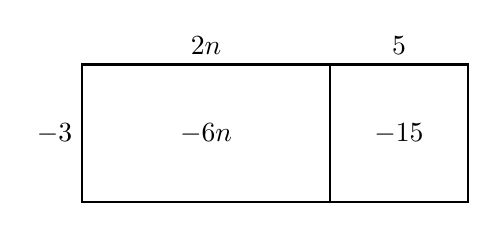
\begin{tikzpicture}[scale=0.7]
  \draw[thick] (0,0) rectangle (7,2.5);
  \draw[thick] (4.5,0) -- (4.5,2.5);
  \node[left] at (0,1.25) {$-3$};
  \node[above] at (2.25,2.5) {$2n$};
  \node[above] at (5.75,2.5) {$5$};
  \node at (2.25,1.25) {$-6n$};
  \node at (5.75,1.25) {$-15$};
\end{tikzpicture}
\end{center}
\end{questionText}
\choiceA{$-3(2n + 5) = -6n + 15$}
\choiceB{$-3(2n + 5) = -6n - 15$}
\choiceC{$-3(2n - 5) = -6n - 15$}
\choiceD{$3(2n + 5) = 6n + 15$}
\correctAnswer{B}
\explanation{The height is $-3$ and the width splits into $2n$ and $5$. Products: $-3 \times 2n = -6n$ and $-3 \times 5 = -15$. So $-3(2n + 5) = -6n - 15$.}
\end{practiceQuestion}

\begin{practiceQuestion}{5-4-q05}{mc}
\begin{questionText}
Solve $\dfrac{2x}{5} - 1 = 3$.
\end{questionText}
\choiceA{$x = 5$}
\choiceB{$x = 10$}
\choiceC{$x = 4$}
\choiceD{$x = 20$}
\correctAnswer{B}
\explanation{Add $1$: $\frac{2x}{5} = 4$. Multiply by $5$: $2x = 20$. Divide by $2$: $x = 10$. Check: $\frac{2(10)}{5} - 1 = 4 - 1 = 3$ \checkmark.}
\end{practiceQuestion}

\begin{practiceQuestion}{5-5-q29}{gsa}
\begin{questionText}
The balance scale tips to the left. Write and solve the inequality that describes this situation.

\begin{center}
\begin{tikzpicture}[scale=0.7]
  % Tilted beam (left side heavier)
  \draw[thick] (0,-0.5) -- (-0.4,-1.2) -- (0.4,-1.2) -- cycle;
  \draw[thick] (-4.5,0.5) -- (4.5,-0.5);
  % Left pan (lower = heavier)
  \draw[thick] (-4.5,0.5) -- (-5.3,0) -- (-3.7,0) -- (-4.5,0.5);
  \draw[thick,fill=funBlue!20] (-5.3,0) -- (-5.3,-0.4) -- (-3.7,-0.4) -- (-3.7,0) -- cycle;
  \node at (-4.5,-0.2) {$2x + 8$};
  % Right pan (higher = lighter)
  \draw[thick] (4.5,-0.5) -- (5.3,-1) -- (3.7,-1) -- (4.5,-0.5);
  \draw[thick,fill=funOrange!20] (3.7,-1) -- (3.7,-1.4) -- (5.3,-1.4) -- (5.3,-1) -- cycle;
  \node at (4.5,-1.2) {$20$};
\end{tikzpicture}
\end{center}
\end{questionText}
\correctAnswer{$2x + 8 > 20$; $x > 6$}
\explanation{The left side is heavier (tips down), so $2x + 8 > 20$. Subtract $8$: $2x > 12$. Divide by $2$: $x > 6$.}
\end{practiceQuestion}

\begin{practiceQuestion}{5-6-q26}{gmc}
\begin{questionText}
Which inequality matches the graph below?

\begin{center}
\begin{tikzpicture}[scale=0.7]
  \draw[thick,->] (-5,0) -- (5,0);
  \foreach \x in {-4,...,4} \draw (\x,0.15) -- (\x,-0.15) node[below] {$\x$};
  \draw[thick,funBlue,<-] (-5,0) -- (1,0);
  \fill[funBlue] (1,0) circle (4pt);
\end{tikzpicture}
\end{center}
\end{questionText}
\choiceA{$x \leq 1$}
\choiceB{$x < 1$}
\choiceC{$x \geq 1$}
\choiceD{$x > 1$}
\correctAnswer{A}
\explanation{Closed circle at $1$ with shading to the left means $x \leq 1$.}
\end{practiceQuestion}

\begin{practiceQuestion}{6-1-q13}{mc}
\begin{questionText}
A floor plan uses the scale $1$ cm $= 2$ m. A closet measures $1.5$ cm by $1$ cm on the plan. What is the actual area?
\end{questionText}
\choiceA{$1.5$ m$^2$}
\choiceB{$3$ m$^2$}
\choiceC{$6$ m$^2$}
\choiceD{$12$ m$^2$}
\correctAnswer{C}
\explanation{Actual dimensions: $1.5 \times 2 = 3$ m and $1 \times 2 = 2$ m. Area: $3 \times 2 = 6$ m$^2$.}
\end{practiceQuestion}

\begin{practiceQuestion}{6-3-q13}{mc}
\begin{questionText}
A circle with radius $5$ cm is described as a condition. How many circles satisfy this condition?
\end{questionText}
\choiceA{None}
\choiceB{Exactly one}
\choiceC{More than one (different positions)}
\choiceD{It depends on the center location}
\correctAnswer{B}
\explanation{All circles with radius $5$ cm are congruent — they have the same shape and size. In terms of the figure itself (ignoring position), there is exactly one such circle.}
\end{practiceQuestion}

\begin{practiceQuestion}{6-4-q15}{mc}
\begin{questionText}
You know two angles of a triangle are $55°$ and $65°$ and a non-included side is $9$ cm. This is an example of:
\end{questionText}
\choiceA{SSS}
\choiceB{SAS}
\choiceC{ASA}
\choiceD{AAS}
\correctAnswer{D}
\explanation{Two angles and a non-included side is AAS (Angle-Angle-Side). This produces a unique triangle.}
\end{practiceQuestion}

\begin{practiceQuestion}{6-5-q19}{sa}
\begin{questionText}
What shape is the cross-section when you cut a sphere through its center?
\end{questionText}
\correctAnswer{A circle (the largest possible circle)}
\explanation{A cut through the center of a sphere produces a great circle — the largest possible circular cross-section, with the same radius as the sphere.}
\end{practiceQuestion}

\begin{practiceQuestion}{6-6-q27}{gmc}
\begin{questionText}
In the diagram below, lines $AB$ and $CD$ intersect at point $O$. Find the value of $y$.

\begin{center}
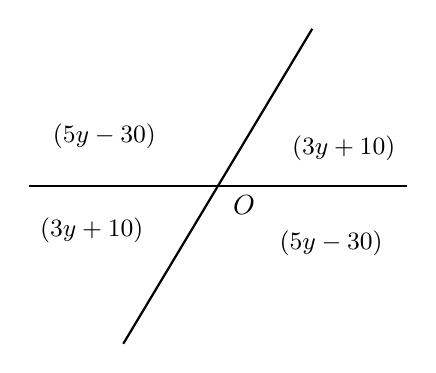
\begin{tikzpicture}[scale=0.8]
  \draw[thick] (-3,0) -- (3,0);
  \draw[thick] (-1.5,-2.5) -- (1.5,2.5);
  \node at (0,0) [below right,xshift=2pt] {$O$};
  \node at (2,0.6) {\small $(3y + 10)°$};
  \node at (-2,-0.7) {\small $(3y + 10)°$};
  \node at (-1.8,0.8) {\small $(5y - 30)°$};
  \node at (1.8,-0.9) {\small $(5y - 30)°$};
\end{tikzpicture}
\end{center}
\end{questionText}
\choiceA{$10$}
\choiceB{$20$}
\choiceC{$25$}
\choiceD{$35$}
\correctAnswer{C}
\explanation{Adjacent angles are supplementary: $(3y + 10) + (5y - 30) = 180$. Combine: $8y - 20 = 180$. Solve: $8y = 200$, $y = 25$.}
\end{practiceQuestion}

\begin{practiceQuestion}{6-7-q24}{sa}
\begin{questionText}
Point $S(-3, -5)$ is reflected over the $x$-axis, then translated right $4$. What are the final coordinates?
\end{questionText}
\correctAnswer{$(1, 5)$}
\explanation{Reflect over $x$-axis: $(-3, -5) \to (-3, 5)$. Translate right $4$: $(-3 + 4, 5) = (1, 5)$.}
\end{practiceQuestion}

\begin{practiceQuestion}{7-3-q01}{mc}
\begin{questionText}
What is the area of a circle with a radius of $3$ cm? Use $\pi \approx 3.14$.
\end{questionText}
\choiceA{$9.42$ cm$^2$}
\choiceB{$18.84$ cm$^2$}
\choiceC{$28.26$ cm$^2$}
\choiceD{$113.04$ cm$^2$}
\correctAnswer{C}
\explanation{$A = \pi r^2 = 3.14 \times 3^2 = 3.14 \times 9 = 28.26$ cm$^2$.}
\end{practiceQuestion}

\begin{practiceQuestion}{7-4-q02}{mc}
\begin{questionText}
What is the first step to find the area of a composite shape?
\end{questionText}
\choiceA{Multiply all the side lengths}
\choiceB{Break it into simpler shapes}
\choiceC{Find the perimeter first}
\choiceD{Measure the diagonal}
\correctAnswer{B}
\explanation{To find the area of a composite shape, break it into simpler shapes (rectangles, triangles, circles, etc.), find each area, and then add or subtract.}
\end{practiceQuestion}

\begin{practiceQuestion}{7-5-q15}{mc}
\begin{questionText}
A triangular prism has two triangular bases each with area $15$ cm$^2$. The three rectangular lateral faces have areas $40$ cm$^2$, $30$ cm$^2$, and $50$ cm$^2$. What is the total surface area?
\end{questionText}
\choiceA{$120$ cm$^2$}
\choiceB{$135$ cm$^2$}
\choiceC{$150$ cm$^2$}
\choiceD{$165$ cm$^2$}
\correctAnswer{C}
\explanation{Two bases: $2 \times 15 = 30$ cm$^2$. Lateral faces: $40 + 30 + 50 = 120$ cm$^2$. Total: $30 + 120 = 150$ cm$^2$.}
\end{practiceQuestion}

\begin{practiceQuestion}{7-6-q21}{sa}
\begin{questionText}
A triangular prism has a triangular base with base $10$ m and height $6$ m. The prism is $8$ m long. What is the volume?
\end{questionText}
\correctAnswer{$240$ m$^3$}
\explanation{$B = \frac{1}{2} \times 10 \times 6 = 30$ m$^2$. $V = 30 \times 8 = 240$ m$^3$.}
\end{practiceQuestion}

\begin{practiceQuestion}{8-1-q03}{mc}
\begin{questionText}
Which sampling method is most likely to produce a representative sample of a school's students?
\end{questionText}
\choiceA{Survey students in the cafeteria during lunch}
\choiceB{Survey every fifth student on an alphabetical class list}
\choiceC{Survey students who volunteer to participate}
\choiceD{Survey only students in honors classes}
\correctAnswer{B}
\explanation{Selecting every fifth student from a list is systematic and gives all students an equal chance, making it more representative.}
\end{practiceQuestion}

\begin{practiceQuestion}{8-3-q21}{sa}
\begin{questionText}
Data set: $4, 6, 7, 8, 10$. The mean is $7$. Find the MAD.
\end{questionText}
\correctAnswer{$1.6$}
\explanation{Deviations from mean: $|4-7|+|6-7|+|7-7|+|8-7|+|10-7| = 3+1+0+1+3 = 8$. MAD $= \frac{8}{5} = 1.6$.}
\end{practiceQuestion}

\begin{practiceQuestion}{8-4-q24}{sa}
\begin{questionText}
Explain one advantage of using IQR instead of range to describe the spread of a data set.
\end{questionText}
\correctAnswer{IQR is not affected by outliers}
\explanation{Range uses only the extreme values, which can be misleading with outliers. IQR measures the middle $50\%$ and gives a more stable picture of typical variability.}
\end{practiceQuestion}

\begin{practiceQuestion}{8-7-q17}{mc}
\begin{questionText}
A double bar graph shows that Store A sold $200$ items in June and $250$ in July. Store B sold $180$ in June and $300$ in July. Which store had a bigger increase?
\end{questionText}
\choiceA{Store A (increase of $50$)}
\choiceB{Store B (increase of $120$)}
\choiceC{They had the same increase}
\choiceD{Neither store increased}
\correctAnswer{B}
\explanation{Store A: $250 - 200 = 50$. Store B: $300 - 180 = 120$. Store B had a bigger increase.}
\end{practiceQuestion}

\begin{practiceQuestion}{9-4-q10}{mc}
\begin{questionText}
A fair die is rolled. Which probability model correctly shows the probability of each outcome?
\end{questionText}
\choiceA{$P(1) = \frac{1}{6}$, $P(2) = \frac{1}{6}$, $P(3) = \frac{1}{6}$, $P(4) = \frac{1}{6}$, $P(5) = \frac{1}{6}$, $P(6) = \frac{1}{6}$}
\choiceB{$P(1) = \frac{1}{6}$, $P(2) = \frac{2}{6}$, $P(3) = \frac{3}{6}$, $P(4) = 0$, $P(5) = 0$, $P(6) = 0$}
\choiceC{$P(\text{even}) = \frac{1}{2}$, $P(\text{odd}) = \frac{1}{2}$}
\choiceD{$P(1) = \frac{1}{3}$, $P(2) = \frac{1}{3}$, $P(3) = \frac{1}{3}$}
\correctAnswer{A}
\explanation{A fair die has $6$ equally likely outcomes, each with probability $\frac{1}{6}$.}
\end{practiceQuestion}

\begin{practiceQuestion}{9-6-q19}{sa}
\begin{questionText}
Two dice are rolled. What is the probability that the sum is $10$ or greater? Write your answer as a fraction in simplest form.
\end{questionText}
\correctAnswer{$\frac{1}{6}$}
\explanation{Sum $10$: $(4,6), (5,5), (6,4)$ — $3$ outcomes. Sum $11$: $(5,6), (6,5)$ — $2$. Sum $12$: $(6,6)$ — $1$. Total: $6$ out of $36$. $P = \frac{6}{36} = \frac{1}{6}$.}
\end{practiceQuestion}

\begin{practiceQuestion}{9-7-q28}{gmc}
\begin{questionText}
The table shows a simulation using random digits $0$--$9$ to model a $30\%$ chance of rain. Digits $0$, $1$, $2$ represent rain. Based on the $10$ trials below, what is the experimental probability of rain?

\begin{center}
\begin{tabular}{|c|c|c|}
\hline
\textbf{Trial} & \textbf{Digit} & \textbf{Rain?} \\
\hline
$1$ & $5$ & No \\
\hline
$2$ & $1$ & Yes \\
\hline
$3$ & $8$ & No \\
\hline
$4$ & $0$ & Yes \\
\hline
$5$ & $3$ & No \\
\hline
$6$ & $7$ & No \\
\hline
$7$ & $2$ & Yes \\
\hline
$8$ & $9$ & No \\
\hline
$9$ & $4$ & No \\
\hline
$10$ & $6$ & No \\
\hline
\end{tabular}
\end{center}
\end{questionText}
\choiceA{$\frac{2}{10} = 0.20$}
\choiceB{$\frac{3}{10} = 0.30$}
\choiceC{$\frac{4}{10} = 0.40$}
\choiceD{$\frac{7}{10} = 0.70$}
\correctAnswer{B}
\explanation{Rain occurred in trials $2$, $4$, and $7$ — that is $3$ out of $10$. $P = \frac{3}{10} = 0.30$.}
\end{practiceQuestion}
